\documentclass[letterpaper]{article} % DO NOT CHANGE THIS
\usepackage[submission]{aaai2027} % DO NOT CHANGE THIS
\usepackage[hyphens]{url} % DO NOT CHANGE THIS
\usepackage{graphicx} % DO NOT CHANGE THIS
\urlstyle{rm} % DO NOT CHANGE THIS
\def\UrlFont{\rm} % DO NOT CHANGE THIS
\usepackage{natbib} % DO NOT CHANGE THIS AND DO NOT ADD OPTIONS
\usepackage{caption} % DO NOT CHANGE THIS AND DO NOT ADD OPTIONS
\frenchspacing % DO NOT CHANGE THIS
\usepackage{booktabs}
\usepackage{amsmath}
\usepackage{amssymb}

\pdfinfo{
/TemplateVersion (2027.1)
}

\setcounter{secnumdepth}{0}

\title{Reducing Loss-Averse Choice in LLMs with Reinforcement Learning}
\author{Anonymous Submission}
\affiliations{}

\begin{document}

\maketitle

\begin{abstract}
Language models can reverse a choice when only the endowed alternative changes.
We study whether post-training can reduce this ownership dependence without
imposing a population-level external ordering over subjective goods. We estimate a
frozen Qwen-derived pseudo-utility from a historical Qwen2.5-7B-Instruct
endpoint and use its sign and magnitude as a two-outcome reward for Group Relative Policy Optimization
(GRPO). Evaluation presents every comparison under both counterfactual
endowments and jointly reports structural loss aversion, status-quo bias,
cross-perspective consistency, and preference preservation. In an exploratory
run, the matched validation estimate of loss aversion falls from 7.637 for the
exact local base to 0.111 after GRPO. On a frozen suite of 50 previously unseen
goods, it falls from 2.209 to 0.226, while consistent choices rise from 0.04\%
to 49.46\%. A frontier-consensus reward ablation yields higher loss aversion
but stronger consistency, exposing a trade-off hidden by any single metric.
The historical-Qwen-derived pseudo-utility agrees with separately elicited
ownership-free preferences on 71.1\% of stable cases, rising to 85.5\% for
high-magnitude comparisons. GSM8K changes by $-0.99$ percentage points with a
paired 95\% interval spanning zero. Two confirmatory seeds both pass the frozen
ID-selection, OOD-50, and GSM8K gates. On a once-opened prospective suite of
49,450 unused configurations, their loss-aversion estimates are 0.031 and
$-0.053$, versus 5.946 for the matched base. These results provide evidence
that targeted post-training can reduce ownership-dependent choice, while
residual status-quo bias and an SFT comparison remain central tests.
\end{abstract}

\section{Introduction}

The answer produced by a language model can depend on how a decision is
framed, even when the underlying alternatives are unchanged. Such sensitivity
matters when models are used as simulated agents or decision aids: changing
which option is described as currently owned should not, by itself, change
which option the model selects. Prior work has documented patterns resembling
human cognitive biases in language models \citep{jones2022capturing,
itzhak2024instructed, echterhoff2024cognitive} and has proposed using language
models as simulated economic agents \citep{horton2023homo}. We focus on a
specific, paired counterfactual: ownership-dependent choice in an
endowment-effect task \citep{kahneman1990endowment,tversky1991loss,
samuelson1988statusquo}.

Mitigating this behavior is not simply a matter of labeling one good
objectively better than another. The goods are heterogeneous and preferences
over them are agent-specific. We therefore ask a narrower question: can
post-training remove the effect of ownership while approximately retaining a
Qwen-family-derived ordering? We estimate a frozen pseudo-utility from a
historical Qwen endpoint's probabilistic choices and use it to construct a
verifiable reward. The reward
changes which good is selected under the two endowments, but does not require a
human or frontier model to define the model's underlying tastes.

Our study makes three contributions. First, we formulate ownership dependence
as a paired evaluation in which the same goods and attributes are presented
under opposite endowments. We report a structural loss-aversion coefficient
$\lambda$, a general status-quo term $\eta$, and direct choice-pattern metrics
together. Second, we introduce a historical-Qwen-derived, magnitude-weighted GRPO
objective and compare its reward source with a frontier-consensus ablation.
Third, we separate configuration validation from a frozen new-goods suite,
match the local base and tuned scoring pipelines, validate the pseudo-utility
against ownership-free preferences, and measure capability retention.

The current evidence is deliberately bounded. The primary configuration result
was used for checkpoint selection and is validation-only. The new-goods suite
was frozen before evaluation and carries the generalization claim. Both
confirmatory seeds pass the frozen ID-selection, OOD-50, and GSM8K gates. The
exploratory run retains substantial $\eta$, and the final submission must
report all seeds and the matched supervised fine-tuning (SFT) baseline rather
than only the best GRPO checkpoint.

\section{Related Work}

\paragraph{Behavioral regularities in language models.}
Behavioral evaluations have exposed framing, status-quo, anchoring, and other
decision patterns in language models \citep{jones2022capturing,
itzhak2024instructed, echterhoff2024cognitive}. This literature emphasizes
functional resemblance rather than attributing human cognition to a model.
Economic-agent studies similarly treat prompts as experimental interventions
whose wording and endowments must be controlled \citep{horton2023homo}. Our
paired design isolates ownership by swapping the endowment while holding the
goods and attribute configuration fixed.

\paragraph{Post-training and preference control.}
Supervised instruction tuning and reinforcement learning from feedback are
widely used to shape model behavior \citep{ouyang2022training}. PPO
\citep{schulman2017ppo}, direct preference optimization
\citep{rafailov2023dpo}, and parameter-efficient adaptation
\citep{hu2021lora} provide complementary approaches to behavioral control.
GRPO replaces PPO's learned critic with group-relative advantages
\citep{shao2024deepseekmath}; DAPO develops related clipping and dynamic
sampling refinements \citep{yu2025dapo}. Our setting differs from open-ended
preference alignment: the response space is binary, the reward is
deterministic, and the target is a frozen historical-Qwen reference rather than a
population-level preference label.

\paragraph{Preferences, utility, and reference dependence.}
We treat each model as a distinct decision-maker with a latent preference
relation over good--attribute configurations. Under completeness and
transitivity, a finite within-agent ordering admits a numerical utility
representation \citep{debreu1954representation}. Stability over the study
window is a modeling assumption \citep{stigler1977degustibus}, not a claim that
language-model responses are context-free; expressed preferences can be
constructed by framing \citep{slovic1995construction}. We therefore separate a
configuration score, using a characteristics-based specification
\citep{lancaster1966new}, from endowment-induced reference dependence
\citep{tversky1991loss}. Probabilistic choices identify a normalized latent
index in the tradition of random-utility discrete-choice models
\citep{mcfadden2000economic,train2009discrete}. This gives a global
\emph{within-agent} ordering on the benchmark, not a universal or welfare
ranking across agents.

\section{Task and Measurement}

\begin{figure}[t]
\centering
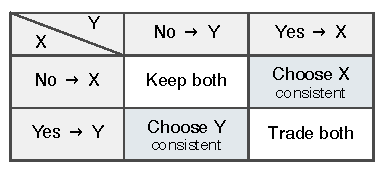
\includegraphics[width=\columnwidth]{figures/task_overview.pdf}
\caption{Paired response map. Swapping only the endowment, the shaded
off-diagonal answer pairs select the same good; diagonal pairs keep or trade
both.}
\label{fig:task}
\end{figure}

\paragraph{Paired perspectives.}
Each configuration contains two goods, $X$ and $Y$, each described by two
ordinal attributes. In the $X$-perspective, the model receives $X$ and is asked
whether to trade for $Y$; in the $Y$-perspective, it receives $Y$ and is asked
whether to trade for $X$. Figure~\ref{fig:task} shows why identical answer
tokens do not imply identical choices: $(\text{No},\text{No})$ keeps the
endowed good in both prompts, whereas $(\text{No},\text{Yes})$ selects $X$
under both endowments.

\paragraph{Structural model.}
For configuration $g=(m,a)$, define the latent index
$v_g=\alpha_m+\beta_a$ and positive score $U_g=\exp(v_g)$. Item 1 and profile
$(1,1)$ are reference categories, so their coefficients are zero. For the
$X$-endowed prompt, the latent keep-versus-trade score is
\begin{equation}
z_i^X=(1+\lambda)U_{X_i}-U_{Y_i}+\eta,
\end{equation}
and the $Y$-endowed equation swaps $X$ and $Y$. The logistic link maps each
score to the probability of keeping the endowed good. The multiplier
$1+\lambda$ captures ownership-specific asymmetry, while $\eta$ captures a
general tendency to preserve the status quo. Ownership neutrality targets
$(\lambda,\eta)=(0,0)$, but the two parameters must be interpreted jointly:
a small $\lambda$ can coexist with substantial choice rigidity absorbed by
$\eta$. This is a task-specific reference-dependent parameterization, not the
canonical prospect-theory value function.

\paragraph{Direct outcomes.}
We also report: (i) \emph{consistency}, the fraction of pairs for which the
same final good is selected under both endowments; (ii) \emph{keep-both}, the
fraction with $(\text{No},\text{No})$; (iii) \emph{trade-both}, the fraction
with $(\text{Yes},\text{Yes})$; and (iv) agreement with a frozen,
ownership-free preference. These measures prevent a low structural coefficient
from masking a constant or otherwise degenerate policy.

\section{Reinforcement Learning with a Historical Qwen Reference}

\paragraph{Historical Qwen reference.}
The trained base is the exact local Qwen2.5-7B-Instruct checkpoint
\citep{qwen2024qwen25}. The reward reference was fitted from a historical
Together-hosted Qwen endpoint using continuous normalized Yes/No probabilities
recovered from top-five first-token log probabilities. The reference is frozen:
it is not recomputed by the exact local base, the GRPO adapter, or later
checkpoints. For each prompt,
``No'' is the keep response. Model A jointly estimates $\lambda$, $\eta$, 99
non-reference item effects, and eight non-reference profile effects by NLS:
\begin{equation}
\begin{split}
\widehat\theta={}&\arg\min_\theta\sum_{i,p}
\bigl[q^{\mathrm{keep}}_{i,p}\,{}-{}\\[-2pt]
&\hspace{32mm}\sigma(z_{i,p}(\theta))\bigr]^2,
\qquad T=1,
\end{split}
\end{equation}
Opposite endowments provide the variation used to separate configuration
scores from ownership asymmetry and the status-quo intercept. We then remove
the latter two components and define
\begin{equation}
\widetilde{\delta}_i=\widehat U_{X_i}-\widehat U_{Y_i}.
\end{equation}
The sign is the historical endpoint's fitted ranking; the magnitude is a
model-normalized separation weight and is not invariant to alternative utility
scales. Thus this is a source-specific pseudo-utility, not the current model's
utility and not objective cardinal
truth. Although
the base model's greedy response is ``No'' in roughly 99\% of endowed prompts,
the continuous probabilities remain informative: item and attribute effects
are well identified, the pseudo-utility has standard deviation $0.94$, and
only 1.6\% of cases are near zero.

We validate the signal against separately elicited ownership-free Qwen
preferences using multiple paraphrases and both display orders. Stable anchors
exist for 6,184 validation configurations and 30,757 training configurations.
The sign of $\widetilde{\delta}$ agrees with these anchors on 71.1\% and 70.8\%
of cases, respectively. Agreement rises with magnitude, reaching 85.5\% when
$|\widetilde{\delta}|>1$. This is convergent evidence across elicitation
framings, not independent human ground truth.

\paragraph{Reward.}
Let $r_i^\star$ be the response that selects the pseudo-utility-preferred good.
For the $X$-perspective, it is ``No'' when
$\widetilde{\delta}_i>0$ and ``Yes'' otherwise; the mapping reverses for the
$Y$-perspective. The reward is
\begin{equation}
\mathcal R(\widehat r_i,\widetilde{\delta}_i)=
\begin{cases}
+|\widetilde{\delta}_i|,&\widehat r_i=r_i^\star,\\
-|\widetilde{\delta}_i|,&\text{otherwise}.
\end{cases}
\label{eq:reward}
\end{equation}
Magnitude weighting concentrates learning on comparisons for which the
historical-Qwen reference ordering is strongest and, empirically, most stable; a
sign-only reward remains the appropriate test of whether the fitted magnitude
adds value.
Within a mixed-response group, unparseable completions receive the negative
reward; an all-identical group is instead zeroed and produces no update.

\paragraph{Training.}
We optimize LoRA adapters \citep{hu2021lora} with GRPO. The exploratory run uses
rank 16, group size 16, rollout temperature 1.5, learning rate $10^{-6}$,
clipping parameter 0.2, KL coefficient 0.04, and maximum completion length
four. Groups with zero reward variance produce no update. Training uses one
NVIDIA A100 40GB GPU and the plain Hugging Face generation path.

\paragraph{Reward-source ablation.}
The ablation replaces the historical-Qwen reference with the mean fitted utility
difference from six frontier models. This tests reward-source aggregation, but the
consensus is also a pseudo-utility rather than ground truth. The two rewards
exhibit a meaningful trade-off: Qwen-derived achieves lower $\lambda$, while the
consensus reward achieves lower $\eta$ and higher choice consistency. Because
utility scales are model-dependent, the mean is an operational aggregation
rule, not a uniquely defined population preference or welfare measure.

\section{Experimental Design}

\paragraph{Data roles.}
Training contains 49,450 configurations (98,900 perspective-specific prompts)
over 100 goods and 4,945 non-trial unordered pairs. Configuration validation
contains 9,890 different configurations over the same goods and pairs: ten
configurations per pair are used for training and two disjoint configurations
are reserved. There are no repeated exact prompts or configurations. Because
validation responses informed pseudo-utility construction and seven
checkpoints were inspected on this split, it is not an untouched final test.

The frozen OOD suite contains 50 previously unseen goods from 10 new
categories, 1,225 pairs, eight configurations per pair, and 9,800 structural
cases. Good names, category names, attribute names, and complete
attribute-value strings have zero exact overlap with the training universe.
The suite was not used for reward construction, training, or checkpoint
selection.

\paragraph{Comparisons and seeds.}
The main comparison includes the exact local base, matched Qwen-derived SFT,
Qwen-derived GRPO seeds 1 and 2, the exploratory seed 42, and the
frontier-consensus GRPO ablation. SFT uses the same prompts, binary targets,
LoRA parameterization, and data budget; it tests whether ordinary supervised
learning is sufficient. Remaining empty cells in Tables~\ref{tab:id-main} and
\ref{tab:ood-main} identify the matched SFT run or metrics that must be
completed before submission.

\paragraph{Checkpoint selection.}
For confirmatory seeds, validation checkpoints were evaluated every 2,000 steps
from 2k to 30k. A checkpoint was eligible only if consistency was at least 0.50
and both structural standard errors are finite and nonzero. Among eligible
checkpoints, selection minimizes
\begin{equation}
d=\sqrt{\widehat\lambda^2+\widehat\eta^2},
\end{equation}
If two distances differ by less than $0.05$, higher consistency is preferred;
if consistency then differs by less than $0.02$, the earlier checkpoint wins.
The rule was frozen before the confirmatory runs. It reproduces the exploratory
8k choice on the seven already evaluated checkpoints, but does not retroactively
remove selection bias from that run.

\paragraph{Scoring and capability retention.}
All structural rows use exact normalized teacher-forced sequence scores for
``Yes'' and ``No'' from native logits and the same nonlinear least-squares
estimator. GSM8K \citep{cobbe2021gsm8k} uses all 1,319 test questions, 8-shot
chain-of-thought prompting, greedy decoding, and a paired comparison. IFEval
\citep{zhou2023ifeval} is the outstanding instruction-following benchmark.
Current structural standard errors are conditional NLS errors; the final
analysis will add pair-aware bootstrap intervals, leave-one-good-out
robustness, estimator-recovery simulation, and across-seed variation.

\section{Results}

% BEGIN AUTO ID_TABLE
\begin{table*}[t]
\centering
\small
\begin{tabular}{lrrrrrrr}
\toprule
Model & $\widehat\lambda$ & $\widehat\eta$ & $W$ & Cons. & Keep & Trade & Pref. agr. \\
\midrule
Exact local base & 7.637 & 1.007 & 0.744 & 0.87\% & 99.13\% & 0.00\% & -- \\
Qwen-derived SFT & -- & -- & -- & -- & -- & -- & -- \\
Qwen-derived GRPO seed 1, step 2k & 0.032 & 0.091 & 0.883 & 66.15\% & 18.24\% & 15.61\% & -- \\
Qwen-derived GRPO seed 2, step 6k & $-0.042$ & 0.659 & 0.910 & 71.76\% & 20.98\% & 7.26\% & -- \\
Qwen-derived GRPO seed 42 (exploratory) & 0.111 & 0.504 & 0.909 & 69.68\% & 24.17\% & 6.16\% & -- \\
Consensus GRPO ablation & 0.177 & $-0.048$ & 0.890 & 90.65\% & 7.84\% & 1.30\% & -- \\
\bottomrule
\end{tabular}
\caption{Configuration-validation results on \texttt{test\_goods}. Every row
uses the same local base weights, 9,890 cases, scorer, and estimator. These are
matched training contrasts, but the post-training estimates are
validation-only because this split informed reward construction and checkpoint
selection. ``Cons.'' selects the same final good under both endowments;
``Keep'' and ``Trade'' denote keep-both and trade-both. $W$ is mean
pseudo-utility alignment,
$w_q=u_{\mathrm{chosen}}/\max(u_1,u_2)$, using one shared frozen Qwen-base
utility reference. It is a descriptive quantity added after the seed
pre-registration. Preference agreement is reserved for the trained policy's
agreement with frozen ownership-free preferences, not the 71.1\% reward-signal
validation. Dashes mark required unfinished runs or metrics.}
\label{tab:id-main}
\end{table*}
% END AUTO ID_TABLE

The exploratory Qwen-derived run reduces validation
$\widehat\lambda$ from 7.637 to 0.111 under a fully matched pipeline. Its
$\widehat\eta=0.504$ and 24.17\% keep-both rate show that general status-quo
rigidity remains, while $W$ rises from 0.744 to 0.909. The consensus ablation
has a higher $\widehat\lambda=0.177$ but near-zero $\widehat\eta$, $W=0.890$,
and 90.65\% consistency. Thus neither reward dominates across outcomes, and
ranking models on $\lambda$ alone would obscure the behavioral difference.

% BEGIN AUTO OOD_TABLE
\begin{table*}[t]
\centering
\small
\begin{tabular}{lrrrrrr}
\toprule
Model & $\widehat\lambda$ & $\widehat\eta$ & Cons. & Keep & Trade & Pref. agr. \\
\midrule
Exact local base & 2.209 & 5.358 & 0.04\% & 99.96\% & 0.00\% & -- \\
Qwen-derived SFT & -- & -- & -- & -- & -- & -- \\
Qwen-derived GRPO seed 1, step 2k & 0.259 & 0.323 & 50.44\% & 38.71\% & 10.85\% & -- \\
Qwen-derived GRPO seed 2, step 6k & 0.064 & 0.593 & 59.83\% & 31.10\% & 9.07\% & -- \\
Qwen-derived GRPO seed 42 (exploratory) & 0.226 & 0.790 & 49.46\% & 46.01\% & 4.53\% & -- \\
Consensus GRPO ablation & 0.395 & 0.502 & 64.89\% & 34.74\% & 0.37\% & -- \\
\bottomrule
\end{tabular}
\caption{Frozen 50-good OOD results. OOD models are compared with the OOD base
on the same suite, never with the ID base. Both confirmatory seeds pass the
frozen OOD and non-degeneracy gates. The reward-source rows illustrate a
trade-off between $\widehat\lambda$, $\widehat\eta$, and consistency.
Dashes mark required unfinished runs or metrics.}
\label{tab:ood-main}
\end{table*}
% END AUTO OOD_TABLE

\paragraph{New-goods generalization.}
On the frozen OOD suite, the exact local base is almost entirely
endowment-locked: 99.96\% of paired cases keep both goods. Its
$\widehat\lambda=2.209$ must therefore be read with the very large
$\widehat\eta=5.358$. The exploratory Qwen-derived policy lowers
$\widehat\lambda$ to 0.226 and raises consistency to 49.46\%, but still keeps
both goods in 46.01\% of pairs. The consensus policy reaches 64.89\%
consistency with $\widehat\lambda=0.395$ and $\widehat\eta=0.502$. This
confirms a reward-source trade-off rather than universal dominance.

\paragraph{Prospective unused configurations.}
After checkpoint selection and the OOD-50/GSM8K verdict were complete, we
opened a prospective suite containing 10 previously unused configurations for
each of the 4,945 familiar goods pairs. On its 49,450 cases, the matched base
has $\widehat\lambda=5.946$ (SE 0.192), while selected seeds 1 and 2 have
$0.031$ (0.007) and $-0.053$ (0.005). Their consistencies are 65.92\% and
71.61\%, versus 0.76\% for the base. This supports within-benchmark
configuration generalization; it is not an unseen-goods result.

\paragraph{Configuration sensitivity.}
The validation configurations are behaviorally consequential rather than
cosmetic. First-differencing the two reserved configurations within each goods
pair and perspective yields a pair-clustered joint test of
$\chi^2(8)=5{,}097.22$; a leave-one-good-out calculation gives
$\chi^2(8)=756.05$. Attribute profiles explain 48.8\% of within-pair,
within-perspective variation, changing the hard response in at least one
perspective for 42.18\% of pairs. Adding attributes reduces pair-grouped
cross-validation MSE by 47.43\%. These results support generalization to
unseen configurations of familiar goods and pairs; they do not by themselves
establish unseen-goods transfer.

% BEGIN AUTO CAPABILITY_TABLE
\begin{table}[t]
\centering
\begin{tabular}{lrr}
\toprule
Model & GSM8K & IFEval \\
\midrule
Exact local base & 86.88\% & -- \\
Qwen-derived GRPO seed 42 & 85.90\% & -- \\
Confirmatory paired base & 86.81\% & -- \\
Qwen-derived GRPO seed 1, step 2k & 86.66\% & -- \\
Qwen-derived GRPO seed 2, step 6k & 86.50\% & -- \\
\bottomrule
\end{tabular}
\caption{Capability retention. GSM8K uses a paired 1,319-item evaluation:
$\Delta=-0.99$ percentage points, paired bootstrap 95\% CI
$[-2.12,+0.15]$, and exact McNemar $p=0.111$. IFEval is pending.}
\label{tab:capability}
\end{table}
% END AUTO CAPABILITY_TABLE

\paragraph{Capability retention.}
The exploratory model is 0.99 percentage points below the matched base on
GSM8K. Confirmatory seed 1 changes accuracy by $-0.15$ percentage points
(95\% CI $[-1.14,+0.83]$), and seed 2 by $-0.30$ points
(95\% CI $[-1.44,+0.83]$). All paired intervals span zero, so the evidence
supports ``no clear change,'' not identical capability. IFEval remains required.

\section{Limitations and Broader Impact}

The pseudo-utility reflects a historical hosted Qwen endpoint's fitted ordering,
not the current local base or trained policy, and not welfare, human preference,
or objective value. Its ownership-free
validation is convergent evidence from the same model family. Its cardinal
magnitude additionally depends on the fixed link scale and exponential
specification. The primary ID
result is validation-only because the split informed the reward and checkpoint
choice. Two confirmatory seeds pass the frozen rule, but their different
$\eta$ values show material training variation; the matched SFT baseline is
not yet available. Conditional NLS errors do not capture shared-good dependence or
seed variation. Raw claim-carrying predictions and selected adapters must be
included in the anonymous code/data package, not merely referenced by
checksums.

The structural coefficient is task- and parameterization-specific. We do not
claim that loss aversion is eliminated, that $\eta$ is eliminated, that the
model is superior to humans, or that it outperforms all frontier models. In
particular, commonly cited human coefficients arise from different tasks, and
our endowed-good multiplier is $1+\lambda$. A useful outcome of this work is a
more disciplined way to audit and modify framing sensitivity while preserving
multiple behavioral diagnostics; a risk is that targeted post-training can
silently replace preferences or degrade capabilities if those outcomes are not
measured.

\section{Conclusion}

Reinforcement learning with a frozen historical-Qwen reference offers a direct way to reduce
ownership-dependent choice while retaining a frozen historical-Qwen reference
anchor. The exploratory results show large matched reductions in
structural ownership dependence on both configuration validation and frozen
new goods, alongside residual status-quo bias and reward-source trade-offs.
Two confirmatory seeds pass the frozen selection, OOD-50, and GSM8K gates.
The remaining decisive tests for the final claim are a matched SFT baseline,
robust pair- and good-aware inference, IFEval, and a complete
anonymous reproducibility package.

\bibliography{references}

\end{document}
